\chapter{算法应用——Bin-Picking}
\label{chap:app}
本章主要介绍3D-MRAI算法的实际应用——Bin-Picking。首先介绍一下Bin-Picking相关背景,以及近些年的具体研究与发展;然后详细介绍基于3D-MRAI算法所开发的一套解决Bin-Picking问题的视觉系统,包括硬件的选型、开发环境、系统的框架设计以及算法的具体实现;最后介绍了针对所开发的Bin-Picking视觉系统,进行了随机抓取的实验,测试了系统抓取的成功率以及系统的抓取速度。

\section{Bin-Picking背景与现状}
使用机器人分拣散乱的工件的问题,在学术上我们称之为Bin-Picking,Bin-Picking并不是一个崭新的问题,学术上对这个问题的研究以及有了五十多年的历史。典型的Bin-Picking系统主要包括三部分:机器人、视觉检测模块和计算机控制模块。其中,视觉检测模块是整个Bin-Picking系统的核心部分,通过视觉检测模块对存放散乱工件的物料箱进行分析,获取目标工件的位姿,计算机控制模块根据视觉检测模块的检测结果规划机器人的运动路径,然后机器人执行完成工件的抓取。

传统的Bin-Picking中检测估计目标工件的算法大致可以分为两类:一类是基于特征匹配的算法,另一类是基于模板匹配的算法。基于特征匹配的算法,通过某些特征描述目标工件,如边角、空洞等特征,然后通过分析特征在空间中的旋转变换和平移变换来估计目标零件的位姿。这一类方法受工件纹理或者结构以及传感器的精度影响很大。另外一类基于模板匹配的方法的精度受限与模板的数量,要获得较高的精度就需要大量的模板,而大量的模板会造成算法运行时间过长。

工业上用于解决Bin-Picking问题的视觉系统也有许多,如图\ref{fig:bin-picking-sys}所示。日本的Fanuc公司推出了基于iRVision的Bin-Picking系统,该系统通过四个相机进行三维视觉重建,然后进行目标定位\cite{connolly2007new}。德国的ISRA Vision公司推出了3D Shape Scan系统,丹麦的Scape Technologies公司推出了Scape-Tech Discs系统,德国的Sick公司退出了PLB-500系统,诸如类似的Bin-Picking系统还有许多,这些Bin-Picking系统的价格大多二十万以上,并且抓取成功率和速度也往往难以满足客户需求,因此工业上还是缺少成熟的、价格便宜的、抓取成功率高、速度快的Bin-Picking解决方案。
\begin{figure}[ht]
  \centering
  \subfloat[Fanuc的iRVision系统]{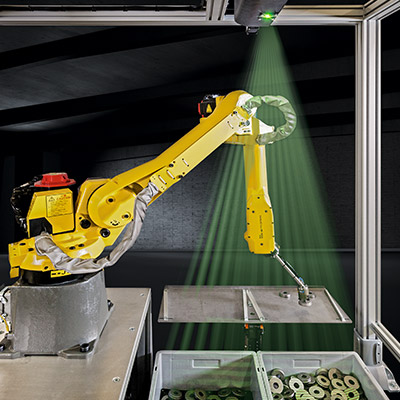
\includegraphics[width=6cm]{fanuc}}
  \hskip1.5cm
  \subfloat[ISRA Vision的3D Shape Scan系统]{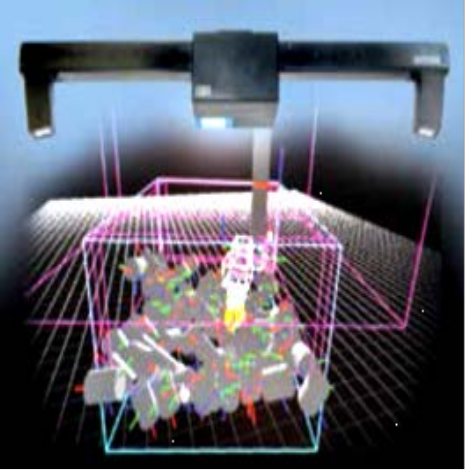
\includegraphics[width=6cm]{3dshape}}
  \vfill
  \subfloat[Scape Technologies的Scape-Tech Discs系统]{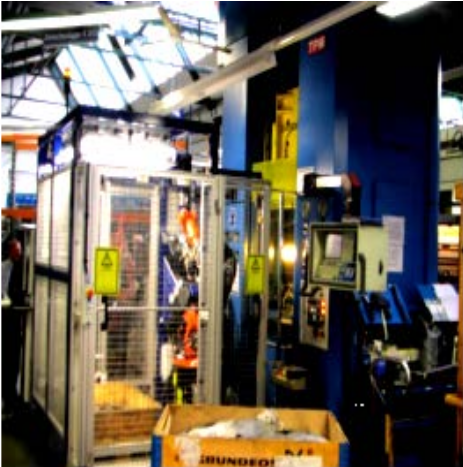
\includegraphics[width=6cm]{scapetech}}
  \hskip1.5cm
  \subfloat[Sick的PLB-500系统]{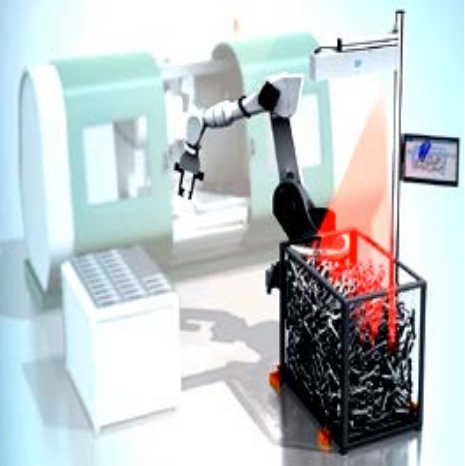
\includegraphics[width=6cm]{plb500}}
  \caption{工业上典型的Bin-Picking解决方案}
  \label{fig:bin-picking-sys}
\end{figure}

随着近几年一些高性价比的3D相机的出现,如微软的Kinect系列、Intel的RealSense系列,加上近几年深度学习的巨大发展,使得开发一种性价比高的、抓取成功率高的、速度快的Bin-Picking系统成为可能。但尽管深度学习在计算机视觉领域(Computer Vision)有了大量的研究,但在机器人感知(Robot Perception)领域的应用还比较少,因此本文将深度学习在计算机视觉领域内的成果通过一些改进引入到Robot Perception领域,再结合传统的全局点云匹配算法,提除了3D-MRAI算法,可以用于解决Bin-Picking相关问题。此外,本文基于Intel的RealSense SR300相机所提出的对偶RGB-D相机构建也为整个Bin-Picking系统提供了高性价比的相机解决方案。

\section{基于3D-MRAI的随机分拣系统}
\subsection{系统硬件设计}
本文所设计的基于3D-MRAI的随机分拣系统的硬件系统如图\ref{fig:hardware-sys}所示。
\begin{figure}[ht]
  \centering
  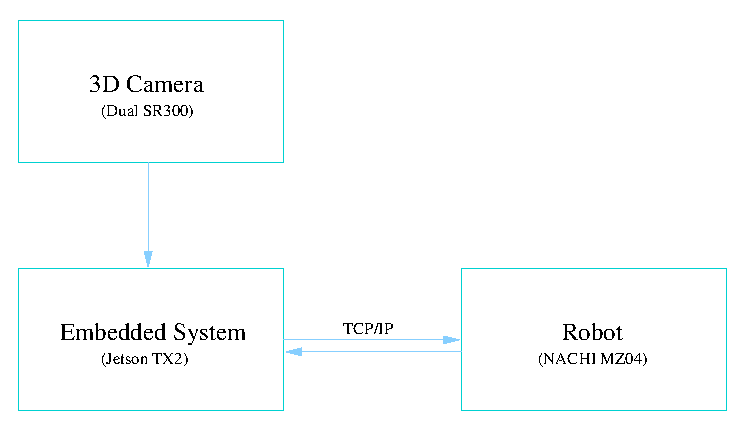
\includegraphics[width=14cm]{hardware-sys}
  \caption{基于3D-MRAI的随机分拣系统硬件框架}
  \label{fig:hardware-sys}
\end{figure}
从图\ref{fig:hardware-sys}可以看出,所设计的随机分拣系统的硬件系统由三个部分构成:相机模块、嵌入式计算模块以及机器人模块。对于相机模块,根据3D-MRAI算法的输入,需要相机能采集RGB-D图像,并且考虑整个系统的响应时间以及价格因此,希望相机模块的采集时间尽可能短,性价比尽可能高,因此选用了以结构光为原理的3D相机,并根据第~\ref{chap:rgbd}~章所设计的对偶RGB-D相机,用两个SR300相机构成了对偶RGB-D相机模块。

嵌入式计算模块选用了搭载了NVDIA公司的Jetson TX2模块的嵌入式计算机,如图\ref{fig:embeded-system},Jetson TX2如图\ref{fig:jetsontx2}所示。
\begin{figure}[ht]
  \centering
  \subfloat[搭载Jetson TX2模块的嵌入式计算机\label{fig:embeded-system}]{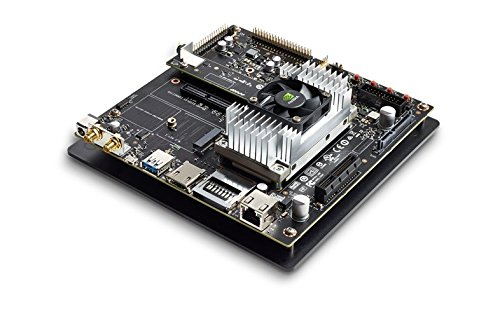
\includegraphics[width=14cm]{embeded-system}}
  \vfill
  \subfloat[Jetson TX2模块\label{fig:jetsontx2}]{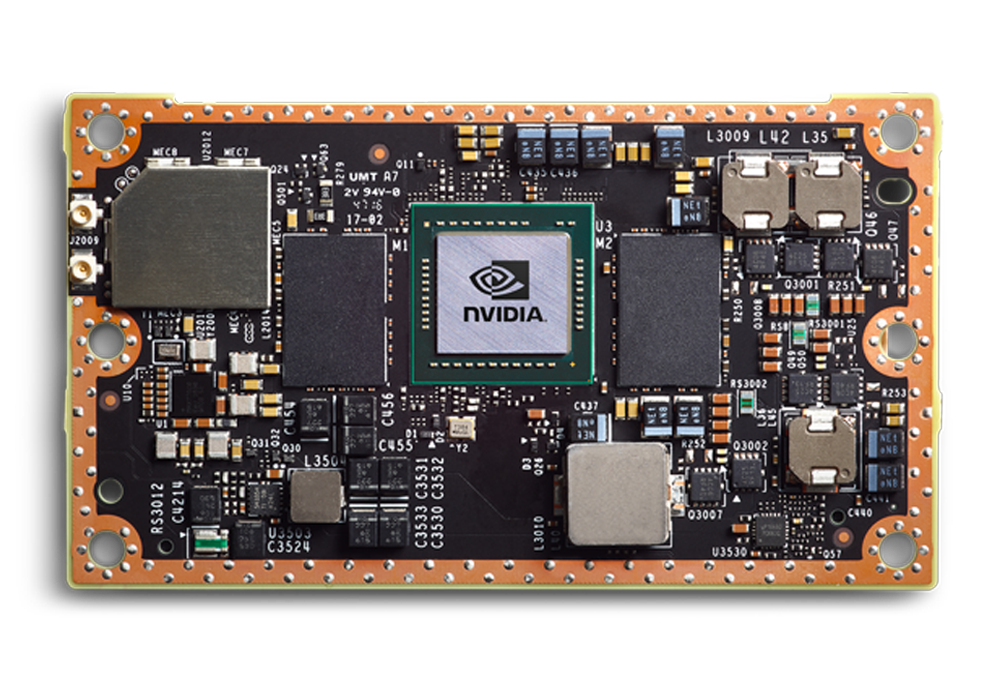
\includegraphics[width=10cm]{jetsontx2}}
  \caption{嵌入式计算模块}
\end{figure}
由于3D-MRAI算法使用了深度神经网络,因此所选用的计算机最好要搭载一块GPU,当然由于模型的训练可以在服务器上完成,只需要在选用的计算机上跑模型的Interface,因此其GPU性能也不需要特别好。另外,考虑到系统需要长时间运行,因此选用了低功耗的嵌入式计算机。所选用的搭载Jetson TX2模块的嵌入式计算机拥有一块Pascal架构的GPU,256个CUDA cores,CPU是HMP Dual Denver加四块ARM A57,内存8G(LPDDR4),还拥有1 Gigabit Ethernet,802.11ac WLAN以及Bluetoothd,在系统计算资源、功耗以及通信上完全满足整个Bin-Picking系统的要求。

机器人模块选用了NACHI的六轴机械臂MZ04,如图\ref{fig:mz04}所示。
\begin{figure}[ht]
  \centering
  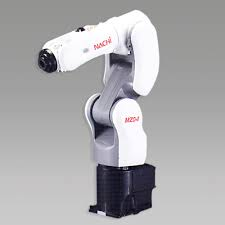
\includegraphics[width=8cm]{mz04}
  \caption{六轴机械臂NACHI MZ04}
  \label{fig:mz04}
\end{figure}
由于一般正常的随机分拣系统所要抓取的工件各种位姿都有,意味着所要抓取的工件有六个自由度,因此所选用的机器人末端至少也要有六个自由度,不然难以完成各种姿态工件的抓取任务,因此选用了工业上常见的六轴机械臂,至于为何选用NACHI的MZ04这个型号,是出于合作方的需要,并不由个人意志决定,当然何种机械臂也不是本文的重点,所设计的视觉算法对机械臂也没什么特殊的要求,因此此处不作详细介绍。

实际搭建随机分拣系统环境如图\ref{fig:bin-picking-env}所示,图中相机固定在支架上,与机械臂构成了eye-to-hand的形式,当然也可以将相机固定在机械臂末端构成eye-in-hand形式,两种固定相机的形式略有不同,但对视觉识别算法那没有影响,只与控制流程和相机与机器人之间的标定有关系,后文会具体介绍到。嵌入式计算机通过相机采集物料箱内的图像,然后运行基于3D-MRAI的视觉系统,得出目标工件位姿,然后规划机械臂路径,通过TCP/IP通信,控制机械臂完成抓取任务,并根据机械臂的运动状态控制整个系统的流程。
\begin{figure}[ht]
  \centering
  %@todo: 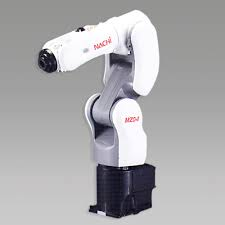
\includegraphics[width=8cm]{mz04}
  \caption{实际搭建随机分拣系统环境}
  \label{fig:bin-picking-env}
\end{figure}

\subsection{系统软件设计}
{\kai 需求分析:}
基于3D-MRAI的随机分拣系统的软件运行在所采用的嵌入式计算机上,主要需要以下几点功能:
\begin{itemize}
\item 图像的采集与处理
\item 与机器人的通信
\item 3D-MRAI算法的实现
\item 机器人相关的处理
\item 可视化界面
\end{itemize}
针对以上几点需求,整个软件分为五个模块,如图\ref{fig:software-module}所示。
\begin{figure}[ht]
  \centering
  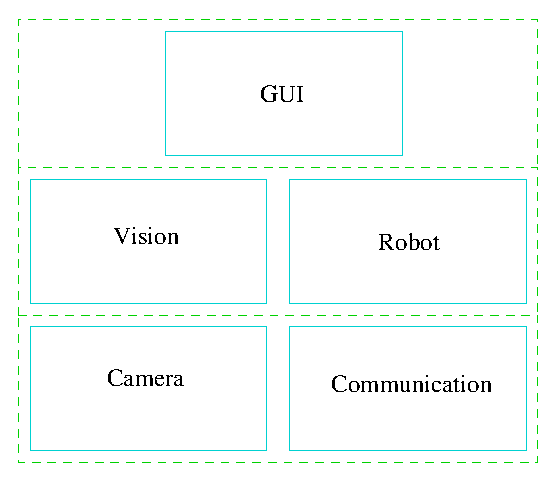
\includegraphics[width=8cm]{software-module}
  \caption{系统软件模块设计}
  \label{fig:software-module}
\end{figure}
Camera模块主要实现对偶RGB-D图像的匹配与合成,旨在提供高质量的RGB-D图像;Communication模块主要实现一个TCP服务器,并且定义了与机器人的通信协议,旨在提供与机器人高效稳定的通讯服务;Vision模块主要实现了3D-MRAI算法,旨在根据输入的RGB-D图像,输出目标工件的位姿;Robot模块主要实现与机器人相关的一些路径规划,根据目标工件的位姿生成机械臂抓取的位姿;GUI模块主要实现对检测结果的可视化,以及一些简单的流程控制。每个模块具体的实现后文会详细介绍。

{\kai 开发环境:}
所采用的嵌入式计算机使用的是嵌入式Linux操作系统,当然由于嵌入式计算机特性,软件的开发主要在通用计算机上,通用计算机也使用了Linux操作系统,这样在编写完成的软件可以无缝拷贝到嵌入式Linux操作系统上,但由于通用计算机和嵌入式计算机的CPU架构不同,将程序拷贝到嵌入式计算机上后,需要重新编译。当然也可以考虑直接在通用计算机上交叉编译嵌入式计算机上的可执行程序,但考虑到调试方便,并且所使用的嵌入式计算机性能强劲,并未使用交叉编译的方式。考虑到系统的性能以及算法的复杂性,整个系统软件使用C++ 11编写,Clang作为编译器,CMake作为自动化编译工具,git作为版本控制,具体如表\ref{tab:dev_env}所示。
\begin{table}[ht]
  \centering
  \begin{tabular}{cc}
    \toprule
    操作系统&Ubuntu 16.04\\
    编译器&Clang 3.8.0 \\
    构建系统&CMake 3.5.1 \\
    版本控制& git 2.7.4 \\
    \bottomrule
  \end{tabular}
  \caption{系统开发环境}
  \label{tab:dev_env}
\end{table}

{\kai 软件依赖:}
系统软件的依赖如下所示:
\begin{itemize}
\item librealsense < 2.0.0
\item OpenCV >= 3.0.0
\item PCL(Point Cloud Library) >= 1.7.0
\item Tensorflow >= 1.2.0
\item Glog >= 0.3.4
\item glfw >= 3.1.2
\end{itemize}
上述所有的软件都是跨平台、开源的软件,librealsense是所使用的RGB-D相机SR300的驱动以及SDK,系统主要使用它获取相机采集的图片;OpenCV是一个基于BSD许可(开源)发行的跨平台计算机视觉库,系统主要使用OpenCV完成对相机采集图像的处理以及对偶RGB-D相机图像的合成与匹配算法;PCL是一个通用的开源点云库,它实现了大量点云相关的通用算法和高效数据结构,涉及到点云获取、滤波、分割、配准、检索、特征提取、识别、追踪、曲面重建、可视化等。支持多种操作系统平台,可在Windows、Linux、Android、Mac OS X、部分嵌入式实时系统上运行,系统主要使用PCL完成一些点云相关的算法;TensorFlow是谷歌基于DistBelief进行研发的深度学习框架,系统主要使用Tensorflow完成3D-MRAI算法中的深度神经网络;Glog是谷歌开发的一个C++语言的应用级日志记录框架,提供了C++风格的流操作和各种助手宏,系统主要使用Glog完成软件的日志记录;glfw是一个OpenGL图形库,系统主要使用glfw完成GUI模块的设计。

\emph{Camera module:}
Camera模块的主要接口是一个虚基类Camera,如图\ref{fig:camera-uml}所示。
\begin{figure}[ht]
  \centering
  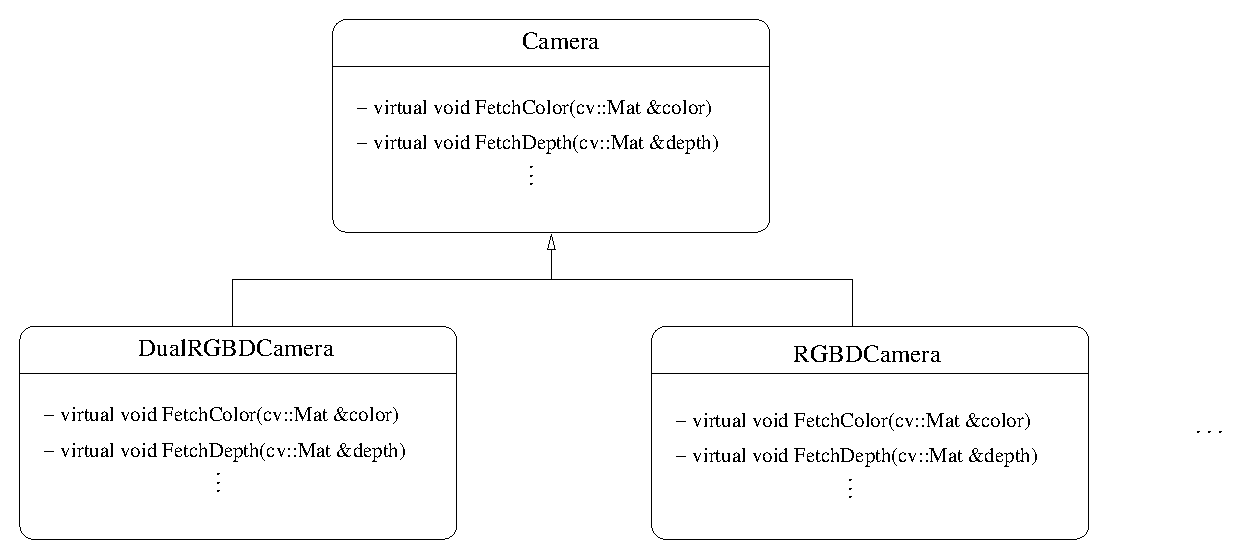
\includegraphics[width=12cm]{camera-uml}
  \caption{Camera module UML}
  \label{fig:camera-uml}
\end{figure}
相机模块通过虚基类Camera定义了一些通用的接口函数,其他具体的相机通过继承这个基类来实现,对于外部使用者来说并不需要关心这些继承Camera类的具体实现,只需要调用Camera中定义的接口即可。整个模块具有很强的扩展性,如增加一个新的相机可以通过增加一个继承Camera的类,外部调用的模块无需改写。实际上,使用何种相机通过设置配置文件可以由用户选择。

\emph{Communication module:}
Communication模块主要使用C++构建了一个TCP服务器,并且规定了通信的协议。讲道理,系统的通讯并不复杂,并且数据量也很小,基本上就视觉系统告诉机器人运动到哪,然后机器人告诉视觉系统是否运动到了目的地这些简单的信息交流。在仔细研究机器人上具体编程后,由于机器人上编程比较单调且繁琐,因此通讯服务的服务器运行在嵌入式计算机上,并且,定义了接收和发送两类信息,发送信息指的是从嵌入式计算机发送到机器人控制器上的信息,接收信息类似。具体定义了一个类模板,如代码\ref{lst:tcp}所示。
\begin{lstlisting}[caption=TCP server template, label=lst:tcp]
template <typename RecvMsgT, typename SendMsgT>
class SyncTCPServer {
 public:
  SyncTCPServer(std::string address = "127.0.0.1", unsigned short port = 8000);

  void WaitingClient() {
    acceptor_->accept(*socket_);
  }

  /**
   * Receive message from client
   * @param msg the received message
   * @return read bytes size
   */
  int RecvMsg(RecvMsgT &msg);

  /**
   * Send message to client
   * @param msg the message will be sent
   * @return write bytes size
   */
  int SendMsg(const SendMsgT &msg);

 private:
  boost::asio::io_service io_service_;
  boost::shared_ptr<boost::asio::ip::tcp::acceptor> acceptor_;
  boost::shared_ptr<boost::asio::ip::tcp::socket> socket_;
};
\end{lstlisting}

\emph{Vision module:}
Vision模块的主要类的UML图如图\ref{fig:vision-uml}所示。
\begin{figure}[ht]
  \centering
  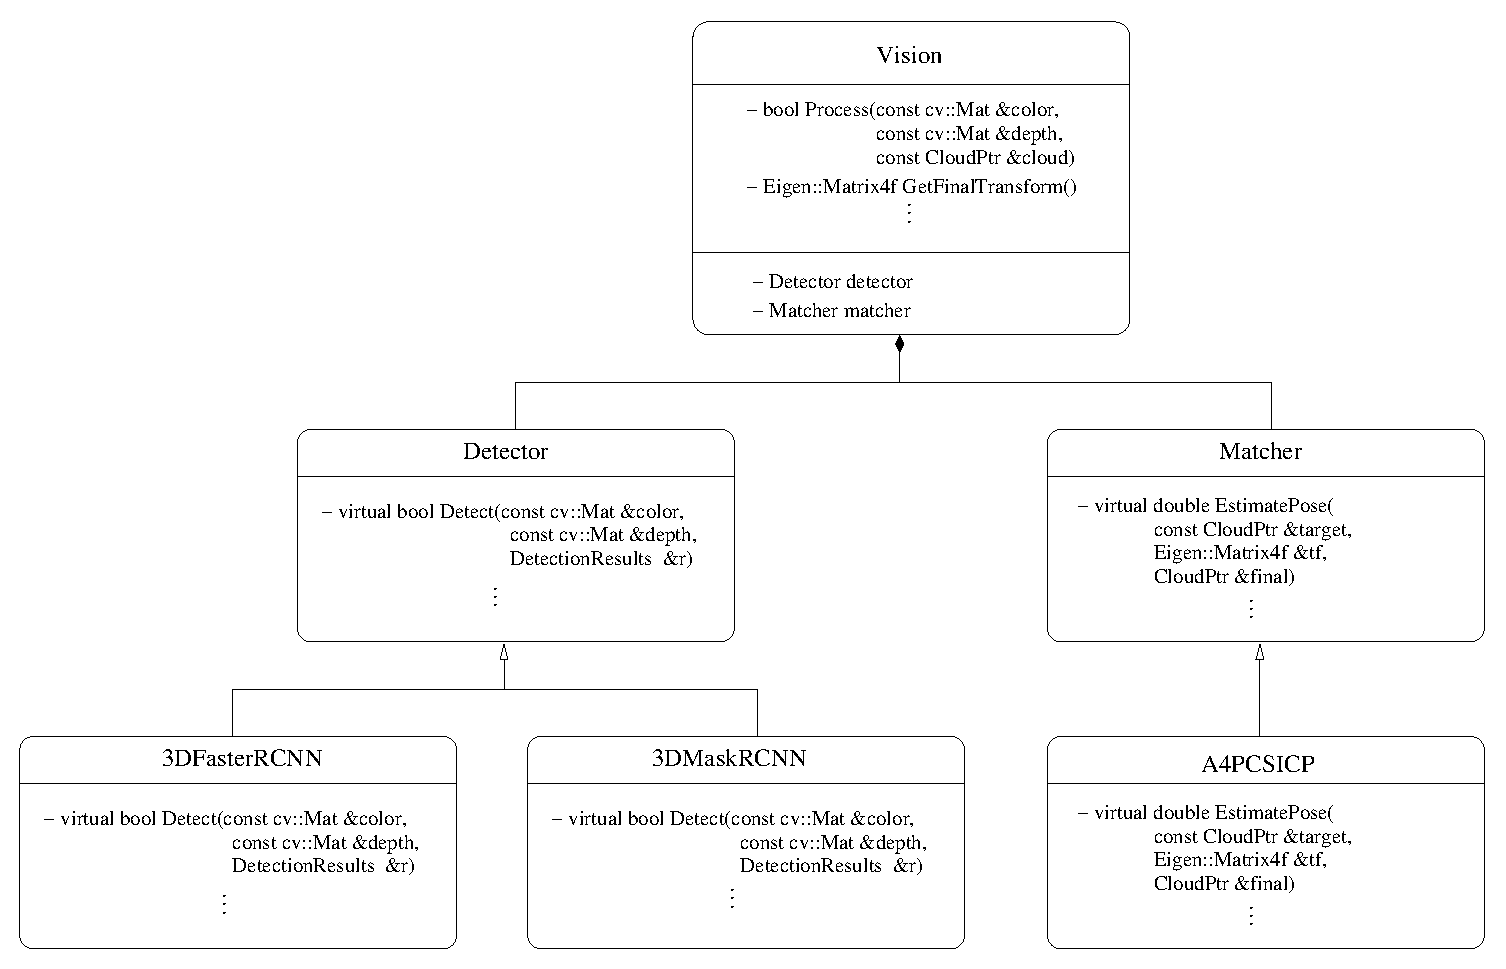
\includegraphics[width=14cm]{vision-uml}
  \caption{Vision module UML}
  \label{fig:vision-uml}
\end{figure}
Vision类提供在图像中找出目标工件位姿的接口,其核心是3D-MRAI算法,因此也有两个模块:Detector和Matcher。Detector和Matcher的设计思想和Camera模块类似,通过定义接口屏蔽具体实现,从提高了程序的扩展性,因为显然可以有多种检测的方法,比如本文就有3D Faster R-CNN和3D Mask R-CNN两种实现,通过这种方式可以在不改动程序代码的情况下,通过配置文件快速切换所想要使用的算法。

Vision类的核心就是3D-MRAI算法,算法具体内容已经在第\ref{chap:pose}~章中详细叙述了,但此处运用于Bin-Picking系统,为了提高系统的效率,针对Bin-Picking这个系统,在实现细节上对3D-MRAI做了些改动,或者说trick。其中最主要的trick是不再对3D Faster/Mask R-CNN中的每个检测结果都去运行A4PCS-ICP算法,取而代之的是通过对每个BBox/Mask提取的点云根据距离工作台的高度排序,从位置最高的点云开始运行匹配算法,满足条件就返回。这么做的原因是,Bin-Picking系统每次抓取只能抓取一个工件,并且,理论上位于物料堆最上面的工件显然最好抓取。增加这个trick后的3D-MRAI算法的流程如算法\ref{alg:modified-mrai}所示,这么做大大减少了视觉系统的运算时间,提高了整个系统的抓取工作效率。除此之外,为了避免抓取时不必要的碰撞,在工件的抓取点附近还会检查有没有障碍物。

TODO:避免碰撞具体实现。

\begin{algorithm}
  \caption{3D-MRAI with Tricks}
  \label{alg:modified-mrai}
  \KwIn{RGB Image $I$, Depth Map $D$, CAD Models $M$}
  \KwOut{Set of Pose and Class $Res$}
  $P\leftarrow \varnothing$\;
  \ForAll {$M_i\in M$} {
    $P\leftarrow \left\{P, CAD2PointCloud(M_i)\right\}$\;
  }
  $H = Depth2HHA(D)$\;
  $Q = Depth2PointCloud(D)$\;
  $Mask, Class \leftarrow 3DMASKRCNN(I, H)$\tcp*{Same with $3DFASTERRCNN$}
  $Q_{sorted}\leftarrow \varnothing$\;
  \ForAll {$m_i\in Mask, c_i\in Class$} {
    $Q_i \leftarrow Crop(Q, m_i)$\;
    $Q_{sorted}\leftarrow {Q_{sorted}, [Q_i, c_i]}$\;
  }
  $SORTBASEDONHEIGHT(Q_{sort})$\;
  \ForAll {$[Q_i, c_i]\in Q_{sort}$} {
    $P_i \leftarrow P(c_i)$\;
    $T_i,S_i\leftarrow A4PCSICP(P_i, Q_i)$\;
    \If {$S_i > S_{min}$} {
      \Return $\left[T_i, c_i\right]$\;
    }
  }
\end{algorithm}

\emph{Robot module:}
Robot模块根据Vision模块输出的工件位姿,将其变换到机器人坐标系下,然后生成轨迹,发送给机器人。由于Vision模块与Robot模块之间是解耦的,Vision模块输出的工件位姿是在相机坐标系下的,为了将相机坐标系下的位姿变换到机器人坐标系下,还需要进行相机和机器人之间的标定(手眼标定),所设计的系统的相机固定在支架上,与机器人分离,因此是一个典型的eye-to-hand calibration。

TODO:具体标定的方法

将工件位姿从相机坐标系变换到机器人坐标系后,便可得机器人抓取的位姿,机器人抓取的位姿与工件的位姿是事先标定好的,并且为了提高抓取的成功率,对一个工件设了多组抓取位姿,根据工件的位姿选取合适的抓取位姿。

\emph{GUI module:}
为了可视化视觉系统的检测情况,设计了GUI模块实时展示检测结果,由于系统中存在3D的点云,因此采用OpenGL库在三维空间中可视化结果,并且可以对程序进行简单的控制。三维可视化的界面如图\ref{fig:gui}所示。
\begin{figure}[ht]
  \centering
  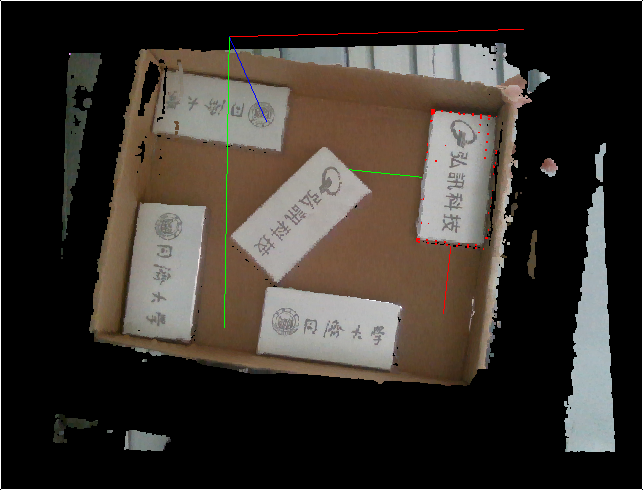
\includegraphics[width=10cm]{gui}
  \caption{视觉系统三维可视化}
  \label{fig:gui}
\end{figure}
三维可视化界面中标出了相机坐标系、检测出要抓取的工件的位姿,整个场景是相机采集到的3D数据,红色部分点云是将目标工件CAD模型变换到所计算得到的工件位姿,因此红色点云与相机采集到的3D目标点云相重合说明视觉系统的检测正确。整个界面是3D的,可以通过鼠标放大、缩小、旋转,也可通过键盘控制视角的前进后退左右移动,全方位360度观察当前检测结果,如图\ref{fig:view-pose}所示,在不同视角下观察检测结果。除此之外,还可以通过键盘保存当前所展示的点云和其他一些数据,方便进一步分析和观察。
\begin{figure}[ht]
  \centering
  \subfloat{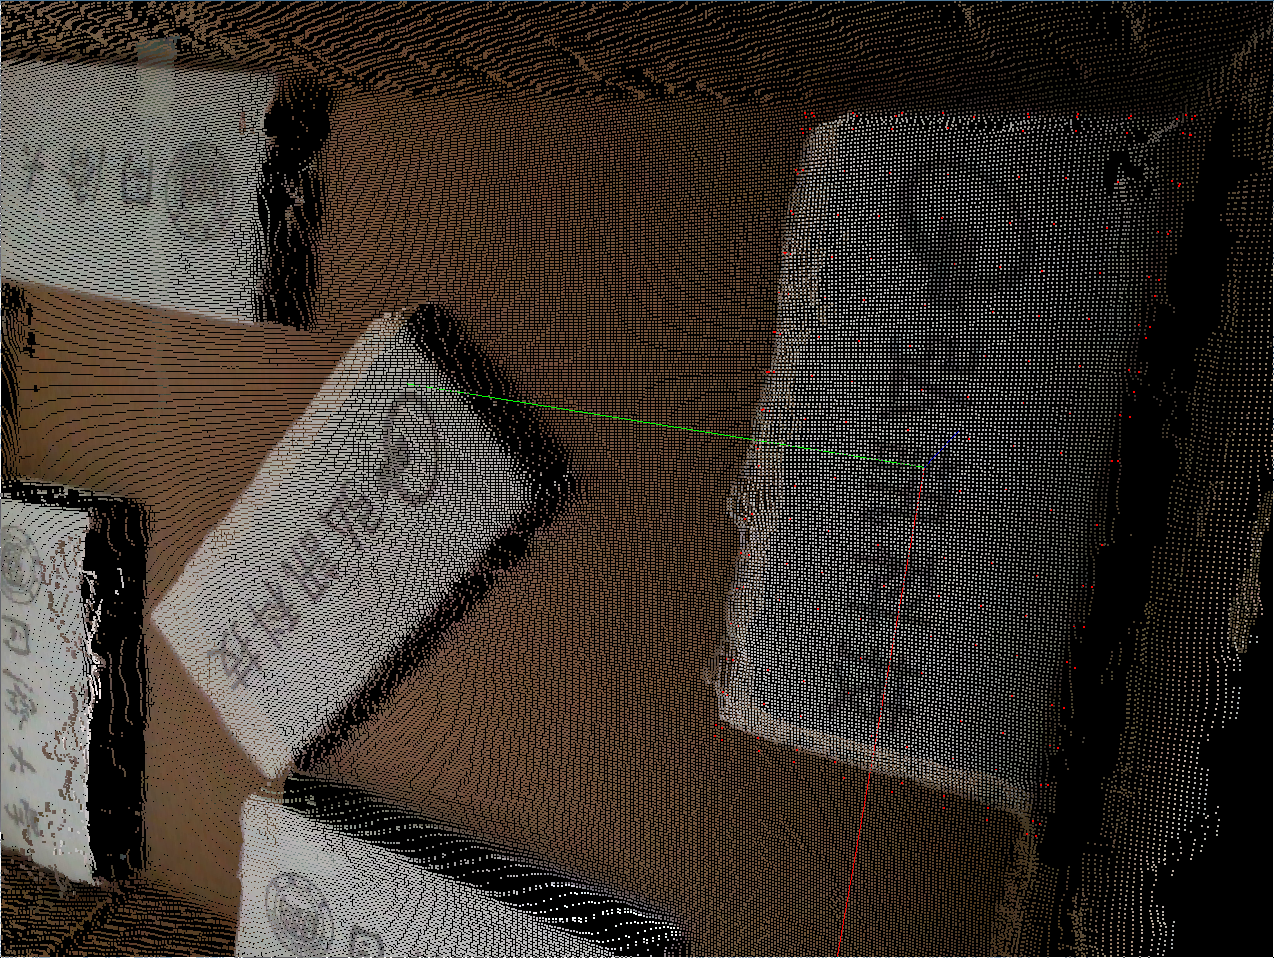
\includegraphics[width=7cm]{ang1}}
  \hfill
  \subfloat{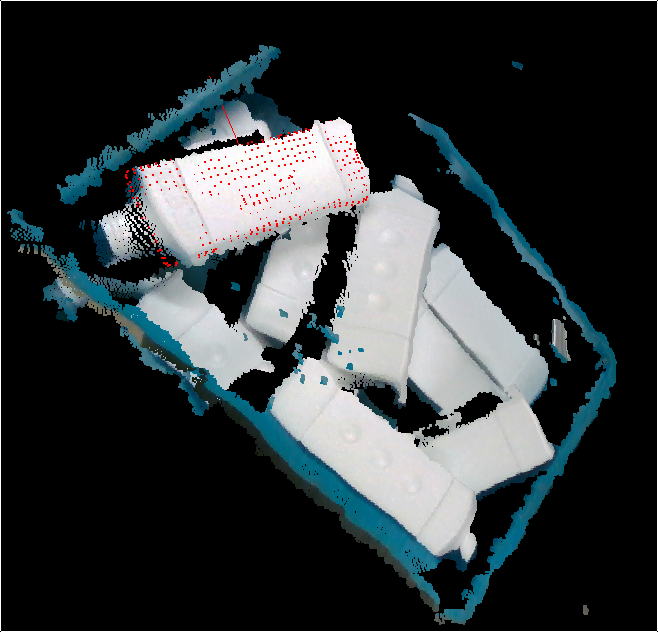
\includegraphics[width=7cm]{ang2}}
  \caption{不同视角下观察检测结果}
  \label{fig:view-pose}
\end{figure}

\section{随机分拣实验}
\subsection{实验内容}
设计的随机分拣实验在所搭建的工作台上进行,在物料箱中随机放慢物料,如图\ref{fig:random-objects}所示,然后运行整个随机分拣系统,将物料中的全部工件分拣到另外一个箱子中,分拣完一箱后,再随机填充物料,一共统计十箱物料的抓取结果。

评价系统的指标主要是系统的抓取成功率:
\begin{equation}
  R = \frac{m}{n}\times 100\%
\end{equation}
其中$n$表示总的抓取次数,$m$表示成功抓取次数。一次成功的抓取是指机械臂成功将一个物料从物料箱中取出,然后放置到另外一个箱子中。除了系统的成功抓取率,为了考察系统的快速性,定义系统的相应时间$T_r$为从机器人请求开始抓取到机器人收到工件位姿,这个时间也是整个软件的响应时间,主要包括了:
\begin{itemize}
\item 相机采集时间
\item 视觉算法计算时间
\item 通讯时间
\end{itemize}
另外再定义机械臂从开始抓取到将物料抓出箱子的时间为抓取时间$T_1$,机械臂从将物料抓出箱子到放置完物料回到抓取起始点的时间为放置时间$T_2$,如果机械臂只要回到抓取起始点就立即请求下一个抓取位姿,则一个工作周期的总时间为
\begin{equation}
  T = T_r + T_1 + T_2
\end{equation}
但是,考虑到系统的相机是固定在支架上的,因此,只要机械臂将物料抓取出箱子就可以请求下一个抓取位姿,所以一个工作周期的总时间可以缩减为
\begin{equation}
  T = T_1 + \max(T_r,T_2)
\end{equation}
对于评价视觉系统来说,我们更关心系统响应时间$T_r$,对于评价整个Bin-Picking系统来说,显然工作周期$T$更重要。
\subsection{实验结果}
所设计的随机分拣系统的硬件系统抓取完十箱物料后,统计每箱的成功率、平均响应时间、平均抓取时间、平均放置时间和平均工作周期,绘制成表\ref{tab:app_res}以及图\ref{fig:app_res}。
\begin{table}[ht]
  \centering
  \begin{tabular}{cccccc}
    \toprule
    &成功率&响应时间$T_r$&抓取时间$T_1$&放置时间$T_2$&工作周期$T$ \\
    \midrule
    1&100\%&711ms&7.6s&4.2s&12.5s \\
    2&100\%&729ms&6.8s&4.2s&11.0s \\
    3&100\%&708ms&6.5s&4.2s&10.7s \\
    4&100\%&701ms&8.1s&4.2s&12.3s \\
    5&100\%&713ms&9.3s&4.2s&13.5s \\
    6&100\%&722ms&6.6s&4.2s&10.8s \\
    7&100\%&693ms&7.9s&4.2s&12.1s \\
    8&100\%&732ms&9.1s&4.2s&13.3s \\
    9&100\%&718ms&8.9s&4.2s&13.1s \\
    10&100\%&723ms&6.9s&4.2s&11.1s \\
    \bf{Avg.}&\bf{100\%}&\bf{715ms}&\bf{7.77s}&\bf{4.20s}&\bf{12.04s} \\
    \bottomrule
  \end{tabular}
  \caption{随机分拣实验结果}
  \label{tab:app_res}
\end{table}
\begin{figure}[ht]
  \centering
  \subfloat[抓取成功率]{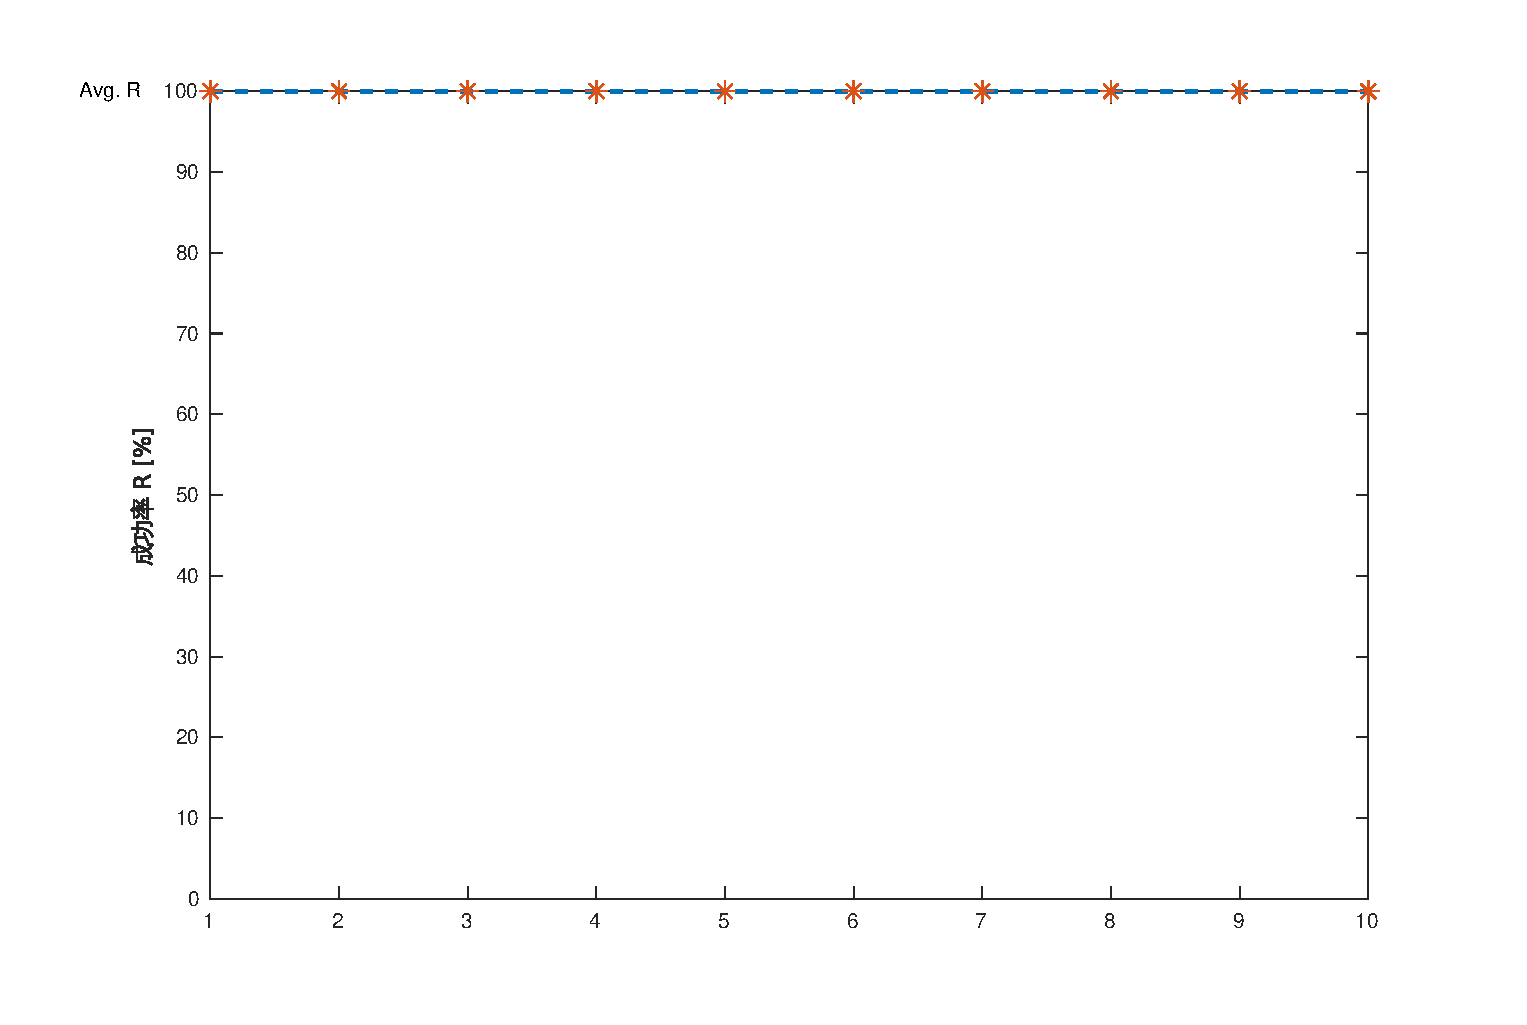
\includegraphics[width=7cm]{app_r}}
  \hskip0.5cm
  \subfloat[响应时间]{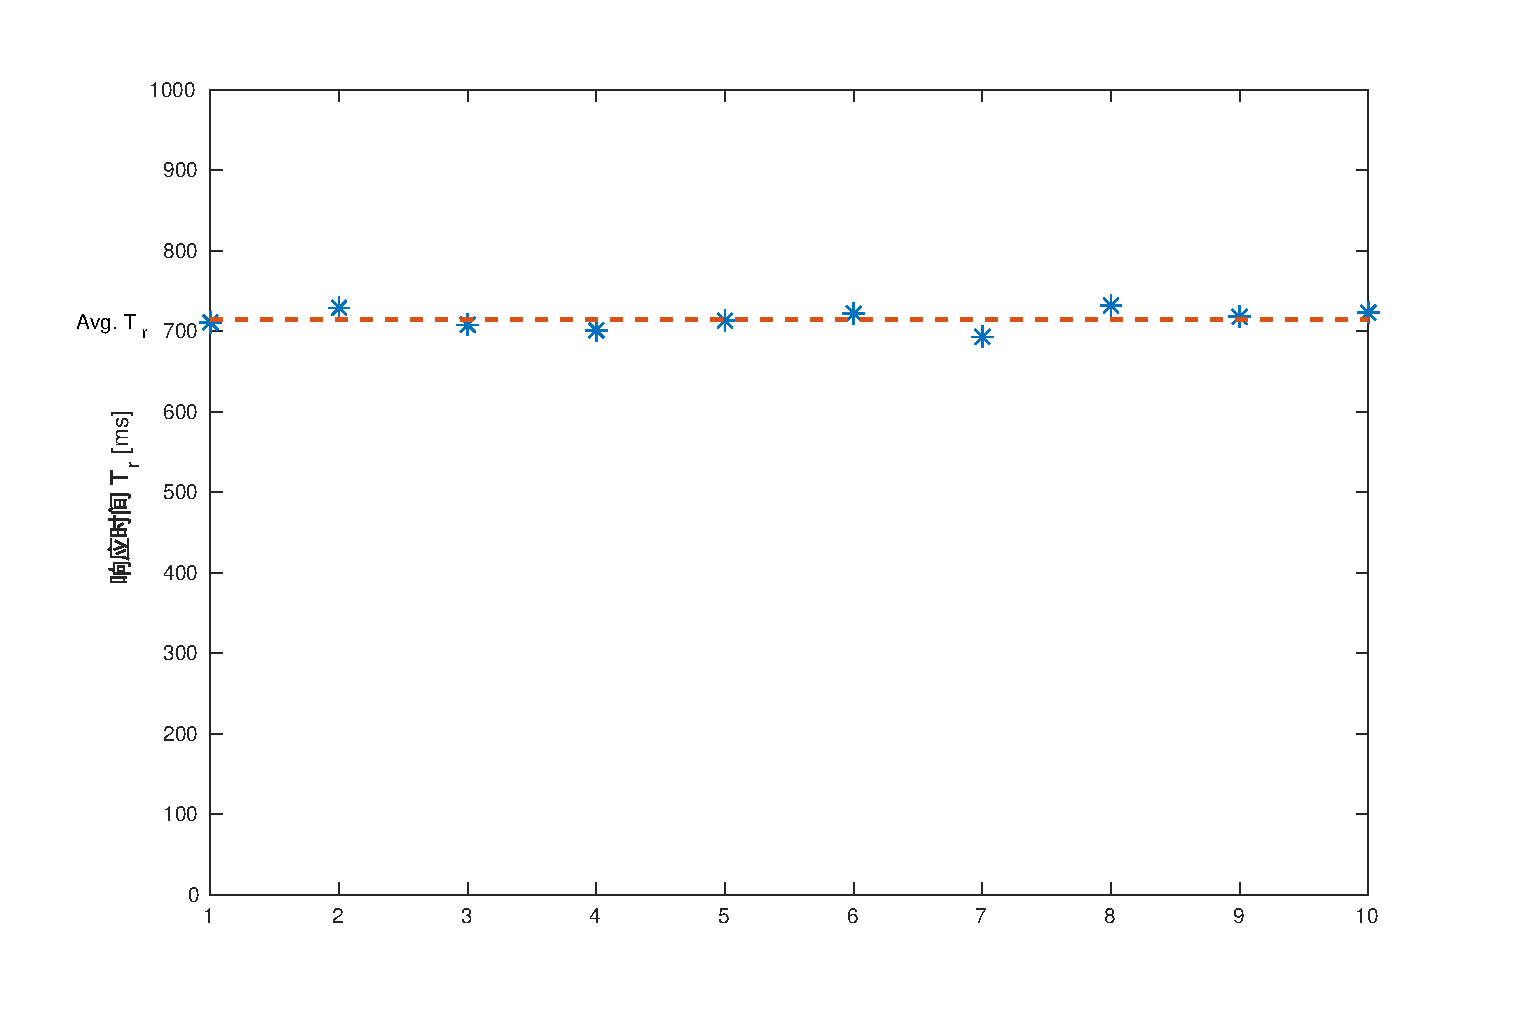
\includegraphics[width=7cm]{app_tr}}
  \vfill
  \subfloat[抓取时间]{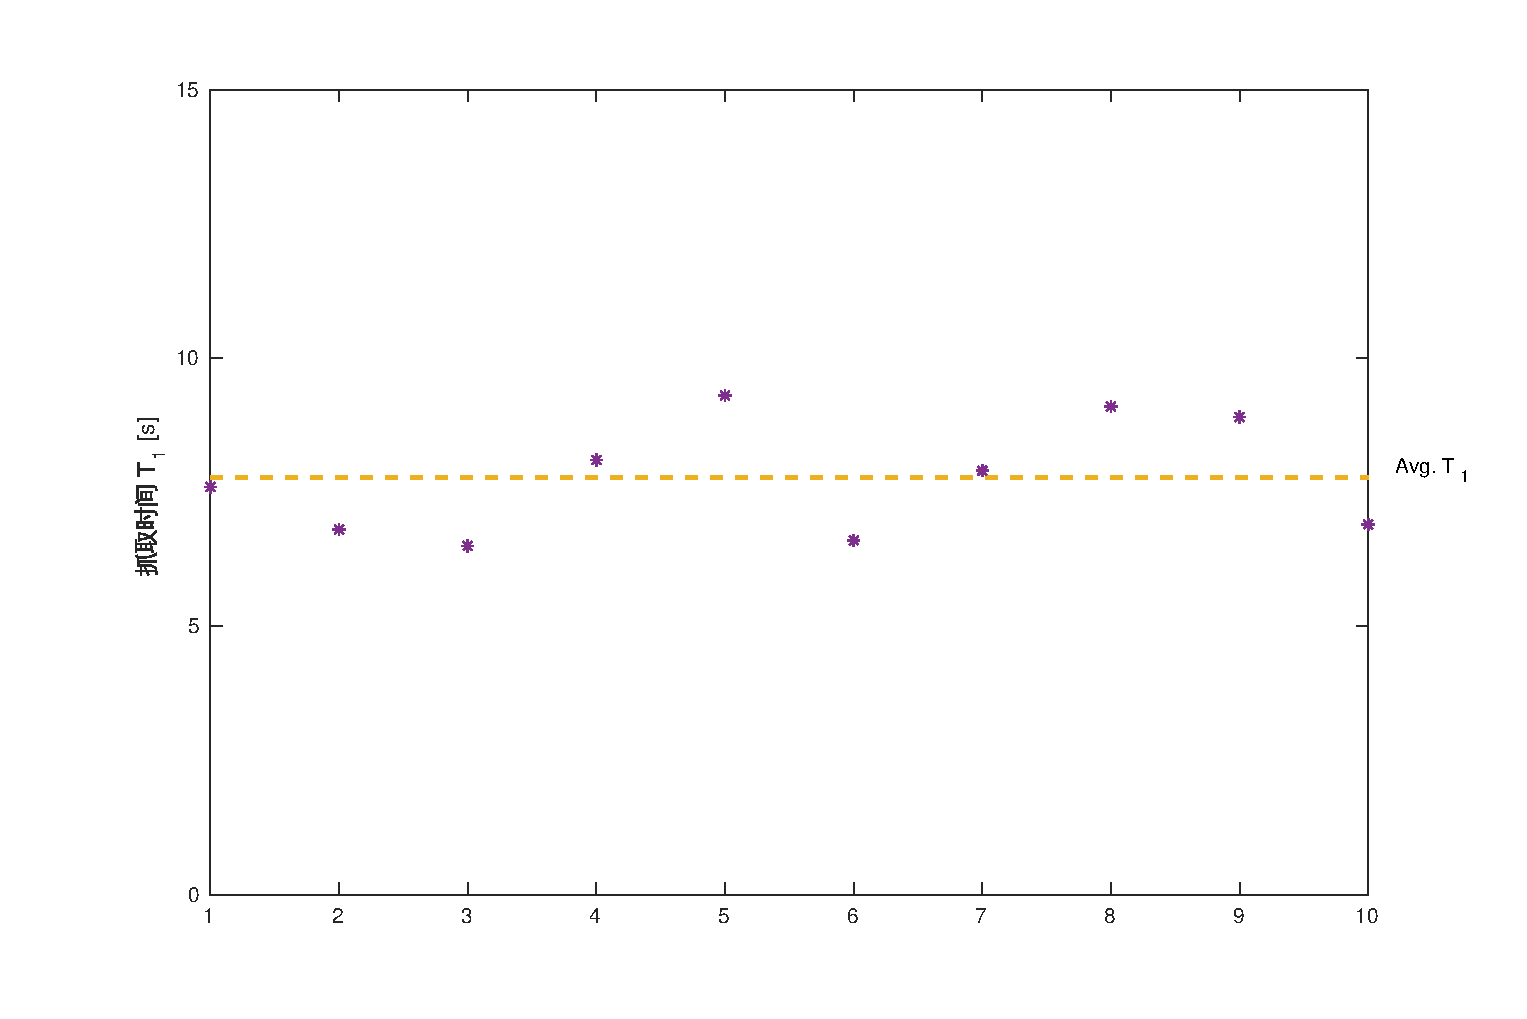
\includegraphics[width=7cm]{app_t1}}
  \hskip0.5cm
  \subfloat[放置时间]{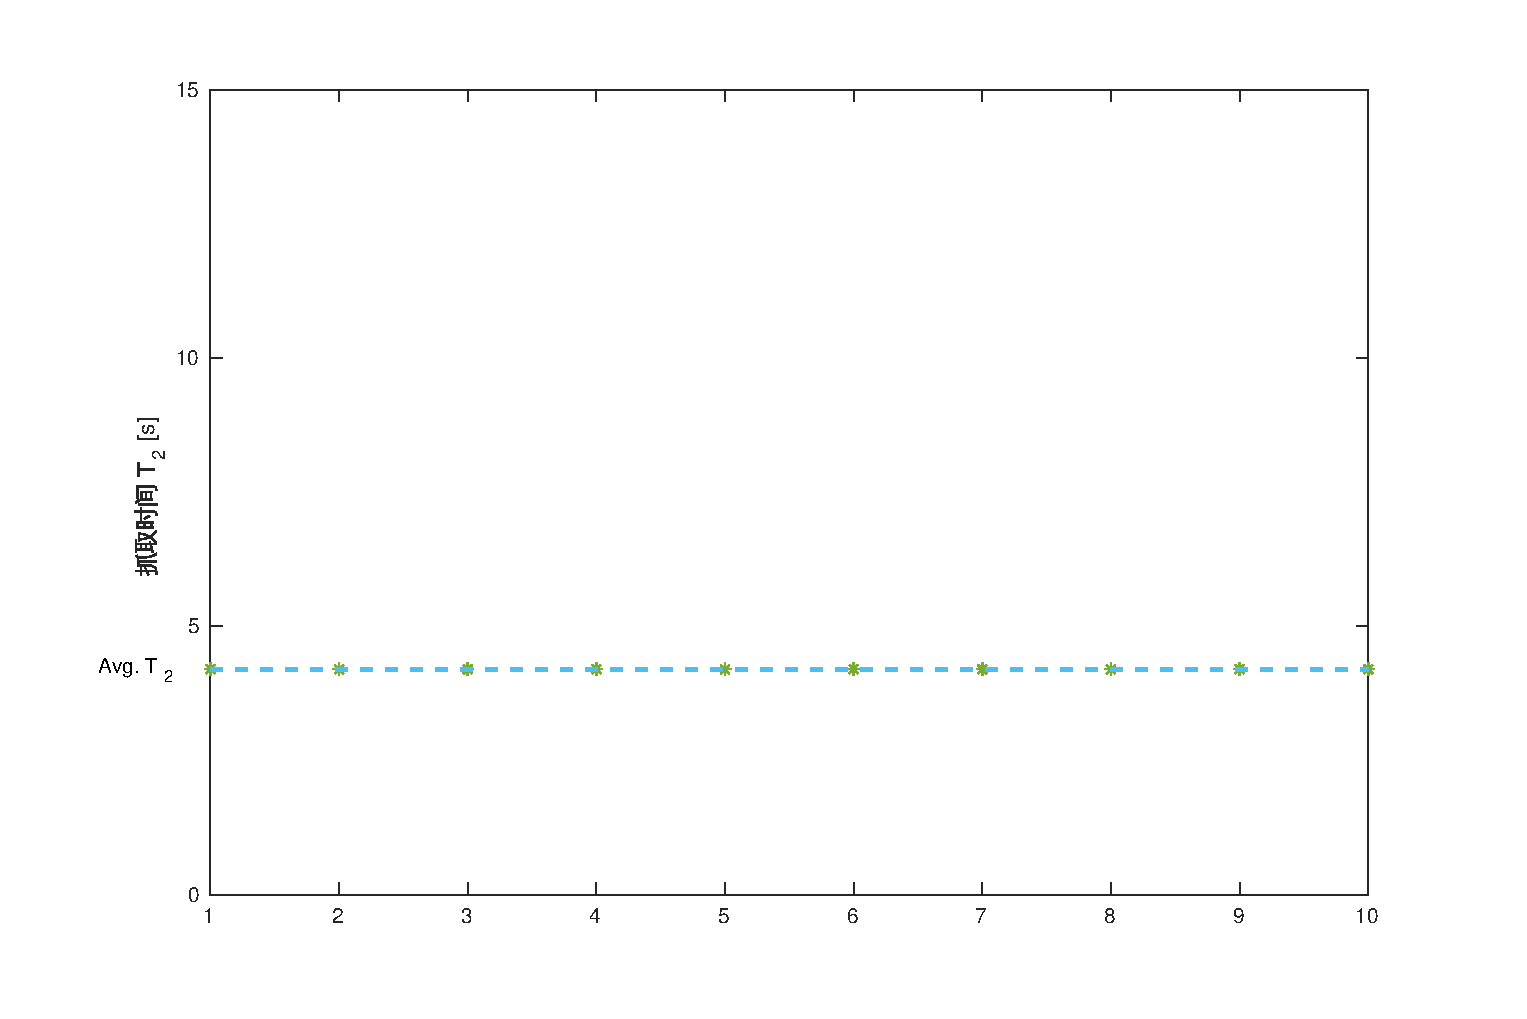
\includegraphics[width=7cm]{app_t2}}
  \vfill
  \subfloat[工作周期]{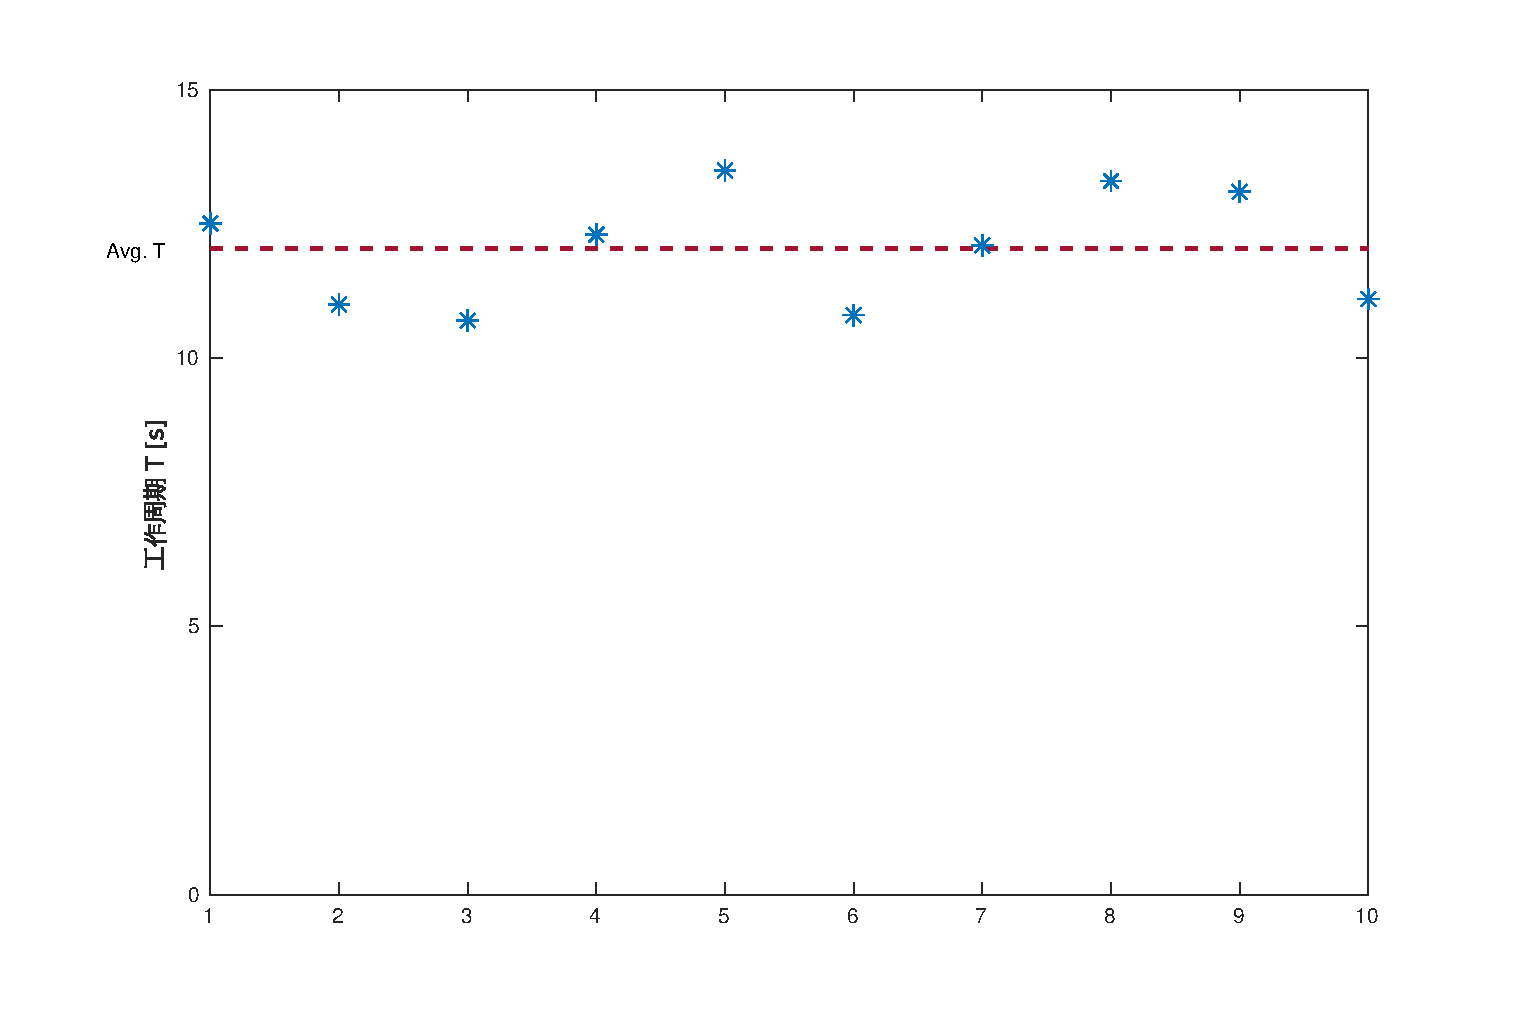
\includegraphics[width=7cm]{app_t}}
  \caption{随机分拣实验结果}
  \label{fig:app_res}
\end{figure}
从表中可以发现所设计的基于3D-MRAI的随机分拣系统的平均抓取成功率为100\%,但理论上随着抓取次数的增加,个人认为系统一定会出现抓取失败的情况,并且实验中所使用的物料也相对单一,不同的物料理论上也会影响视觉的识别效果,因此换一种物料系统的抓取成功率也可能达不到100\%。但总体上来说,此次实验100\%的成功率充分说明了所设计的Bin-Picking视觉系统完全能满足一般随机分拣任务,成功率高。

另外,视觉系统的响应时间为$715ms$左右,分拣系统的工作周期为$12.04s$左右,从表中数据可以发现工作周期基本上为抓取时间和放置时间之和,也就是完全是机械臂运动的时间,除了一开始系统启动时会增加额外的响应时间,但这对真个工作时间来说可以忽律不计,因此,所设计的基于3D-MRAI算法的Bin-Picking视觉系统在时间上完全满足一般分拣任务的要求,实时性高。

\section{本章小结}
本章将3D-MRAI算法应用到实际机器人上,用以解决Bin-Picking随机分拣问题,设计并实现了一个Bin-Picking视觉系统,并进行了抓取实验,实验结果表明,所设计的视觉系统有很高的抓取成功率,并且其响应速度也完全能满足分拣任务的要求。

%%% Local Variables:
%%% TeX-master: "../thesis.tex"
%%% End: